\documentclass[a4paper, 11pt]{article}
\usepackage[top=2cm, bottom=2cm, left=2cm, right=2cm]{geometry}
\usepackage[utf8]{inputenc}
\usepackage[french]{babel}
\usepackage[T1]{fontenc}
\usepackage{lmodern}
\usepackage{graphicx}
\usepackage{caption}
\usepackage{subcaption}
\usepackage{xcolor}
\usepackage{pdfpages}
\usepackage{indentfirst}
\usepackage{hyperref}
\usepackage{float}
\usepackage{listings}

\title{
\includegraphics[scale = 1]{Logos.png} 
\includegraphics[scale = 1.25]{Logo_BCD-1-300x300.png}
\\ [1cm]
{\color{teal}\rule{\linewidth}{1mm}}
\\ [1cm]
\textbf{COMPTE-RENDU \\ PROJET : Modélisation d'une base de données} 
\\ [1cm]
{\color{teal}\rule{\linewidth}{1mm}}
\\ [1cm]
\textbf{HMSN204: \\Informations biologiques et Outils bioinformatiques}\\ [1cm]}
\author{\textit{Auteurs: }\\ \textbf{BATTISTEL} Clémentine \\ \textbf{BOUVIER} Quentin \\ \textbf{KON-SUN-TACK} Fabien \\ \textbf{MARCO} Corentin \\ [0.5cm] \textit{Responsables: } \\ \textbf{ARIGON} Anne-Muriel \\ \textbf{MOUGENOT} Isabelle \\ [1cm] \textsc{Master} Sciences et Numériques pour la Santé\\ \textsc{Parcours} Bioinformatique Connaissances et Données\\ [1cm] \\\textsc{Année universitaire :} 2020-2021}
\date{\today}

\begin{document}
\pagestyle{empty}

\maketitle

\tableofcontents

\newpage
\setcounter{page}{1}
\pagestyle{plain}

\section{Introduction}
\par L'Arabette des dames, plus connue dans le domaine scientifique sous le nom d'\textit{Arabidopsis Thaliana}, est considérée depuis plus de 20 ans comme un organisme modèle de référence pour la recherche biologique, plus particulièrement en génétique. En effet, il s'agit de la première plante au monde dont le génome a été séquencé dans son intégrité, avec un génome de petite taille (seulement 135 Mbp ou 135 \textit{Millions de paires de bases}).
\newpage
\section{Répartition des tâches: Diagramme de Gantt}
\newpage
\section{Modélisation conceptuelle des données}
\subsection{Diagrammes UML}
\begin{figure}[H]
    \centering
    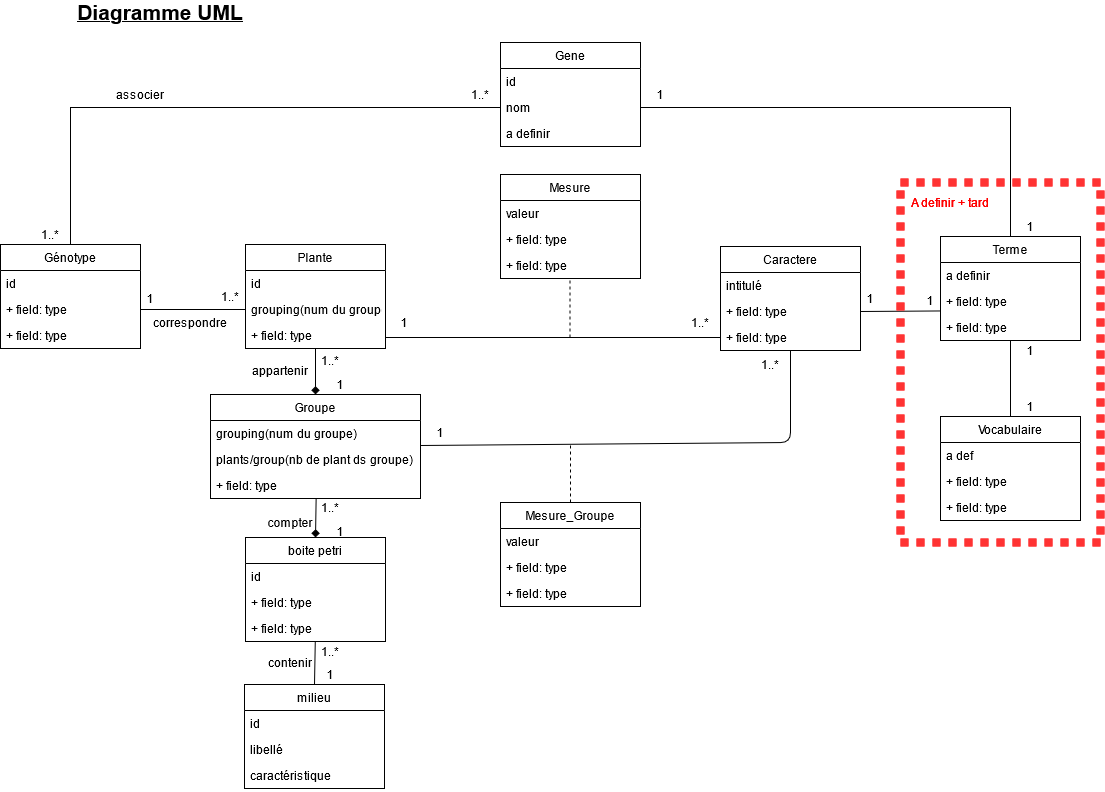
\includegraphics[width=\linewidth]{164839924_120287100013414_6851266838196859948_n.png}
    \caption{Diagramme de classes de la base de données}
    \label{Classes UML}
\end{figure}
\subsection{Choix de la base de données}
\newpage
\section{Implémentation et peuplement de la base de données}
\subsection{Implémentation}
\subsection{Peuplement}
\subsection{Jeu de requêtes}
\newpage
\section{Traitements bioinformatiques: Biopython}
\subsection{Alignement global de séquences par paires}
\subsection{Récupération des séquences à partir du NCBI}
\subsection{Comparaison des alignements avec BLAST}
\newpage
\section{Discussions}
\newpage
\section{Conclusion}
\end{document}
